% Options for packages loaded elsewhere
\PassOptionsToPackage{unicode}{hyperref}
\PassOptionsToPackage{hyphens}{url}
%
\documentclass[
]{article}
\usepackage{amsmath,amssymb}
\usepackage{iftex}
\ifPDFTeX
  \usepackage[T1]{fontenc}
  \usepackage[utf8]{inputenc}
  \usepackage{textcomp} % provide euro and other symbols
\else % if luatex or xetex
  \usepackage{unicode-math} % this also loads fontspec
  \defaultfontfeatures{Scale=MatchLowercase}
  \defaultfontfeatures[\rmfamily]{Ligatures=TeX,Scale=1}
\fi
\usepackage{lmodern}
\ifPDFTeX\else
  % xetex/luatex font selection
\fi
% Use upquote if available, for straight quotes in verbatim environments
\IfFileExists{upquote.sty}{\usepackage{upquote}}{}
\IfFileExists{microtype.sty}{% use microtype if available
  \usepackage[]{microtype}
  \UseMicrotypeSet[protrusion]{basicmath} % disable protrusion for tt fonts
}{}
\makeatletter
\@ifundefined{KOMAClassName}{% if non-KOMA class
  \IfFileExists{parskip.sty}{%
    \usepackage{parskip}
  }{% else
    \setlength{\parindent}{0pt}
    \setlength{\parskip}{6pt plus 2pt minus 1pt}}
}{% if KOMA class
  \KOMAoptions{parskip=half}}
\makeatother
\usepackage{xcolor}
\usepackage[margin=1in]{geometry}
\usepackage{graphicx}
\makeatletter
\def\maxwidth{\ifdim\Gin@nat@width>\linewidth\linewidth\else\Gin@nat@width\fi}
\def\maxheight{\ifdim\Gin@nat@height>\textheight\textheight\else\Gin@nat@height\fi}
\makeatother
% Scale images if necessary, so that they will not overflow the page
% margins by default, and it is still possible to overwrite the defaults
% using explicit options in \includegraphics[width, height, ...]{}
\setkeys{Gin}{width=\maxwidth,height=\maxheight,keepaspectratio}
% Set default figure placement to htbp
\makeatletter
\def\fps@figure{htbp}
\makeatother
\setlength{\emergencystretch}{3em} % prevent overfull lines
\providecommand{\tightlist}{%
  \setlength{\itemsep}{0pt}\setlength{\parskip}{0pt}}
\setcounter{secnumdepth}{-\maxdimen} % remove section numbering
\ifLuaTeX
  \usepackage{selnolig}  % disable illegal ligatures
\fi
\usepackage{bookmark}
\IfFileExists{xurl.sty}{\usepackage{xurl}}{} % add URL line breaks if available
\urlstyle{same}
\hypersetup{
  pdftitle={Informe Polizas},
  pdfauthor={Mathew Cisneros \& Luis Lapo},
  hidelinks,
  pdfcreator={LaTeX via pandoc}}

\title{Informe Polizas}
\author{Mathew Cisneros \& Luis Lapo}
\date{2024-06-13}

\begin{document}
\maketitle

\section{Introduccion (Enofoque del
Analisis)}\label{introduccion-enofoque-del-analisis}

La aplicación de técnicas avanzadas de análisis de datos como la
limpieza de datos, el análisis exploratorio, las series de tiempo y el
clustering k-means en el ámbito de las pólizas de seguros es fundamental
para desentrañar patrones complejos, tomar decisiones informadas y
formular estrategias de negocio efectivas. Estas técnicas permiten a las
aseguradoras no solo cumplir con sus requisitos regulatorios y
operativos sino también adaptarse a un mercado cambiante y a las
necesidades de los clientes.

Para esto vamos a dar una breve explicacion de los metodos usados y las
preguntas o tomas dedecisiones que nos podemos hacer.

\subsection{Preprocesamiento de Datos y Manejo de
Calidad}\label{preprocesamiento-de-datos-y-manejo-de-calidad}

\subsection{Exolicacion del metodo:}\label{exolicacion-del-metodo}

En la fase inicial del análisis, el enfoque principal fue comprender a
profundidad la naturaleza de los datos recopilados. Este proceso implicó
una revisión meticulosa para identificar y determinar valores atípicos
que podrían sesgar los resultados del análisis. Se aplicaron técnicas
estadísticas avanzadas para asegurar una evaluación precisa de estos
valores, facilitando una mejor interpretación de los datos y
estableciendo una base sólida para los análisis subsiguientes.

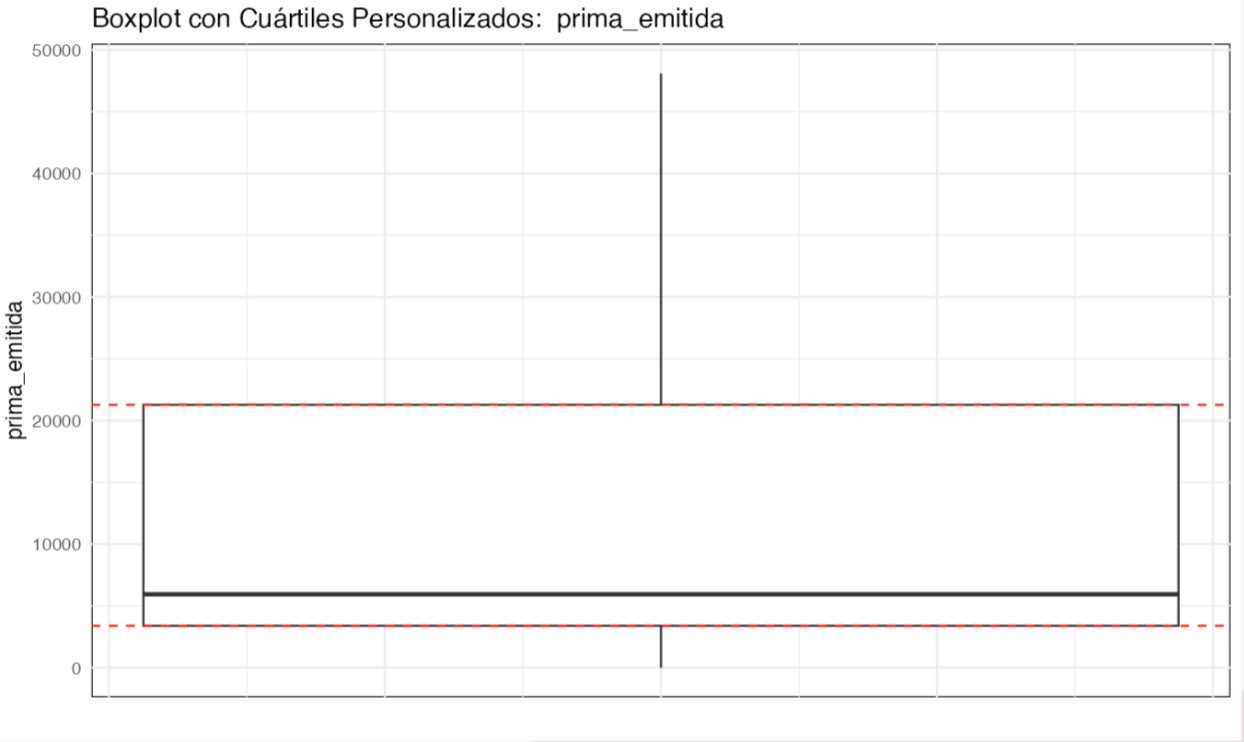
\includegraphics{PHOTO-2024-06-13-15-00-55.jpg}

\subsubsection{Conclusiones y resultados para toma de
decisiones:}\label{conclusiones-y-resultados-para-toma-de-decisiones}

En este caso tomamos el metodo mas comun, usar el rango intercuartilico,
sin embargo tenemos algunas opciones para trtar datos atipicos: -
Estadistica directa: No hace suposiciones estrictas sobre la
distribuciones de los datos - Estadistica Bayesiana: Integra informacion
previa con la evidencia actual para decicir el trato de la variables -
Metodos Bootstrap: Utiliza re.muestreo - Analisis de componentes
principales: Reduccion de la dimensionalidad. Sin embargo hemos aplicado
el mas comun, hemos realizado el diagram de caja y bigotes, tanto en los
datos originales como en los datos alterados. Podemos observar que en
los datos originales existe una cantidad gigante de valores atipicos la
pregunta es que tan importante son estos datos antes de borrarlos o
reemplazarlos.

\subsection{Análisis Exploratorio en Relación a la Sucursal y el Ramo
Comercial}\label{anuxe1lisis-exploratorio-en-relaciuxf3n-a-la-sucursal-y-el-ramo-comercial}

\section{Explicacion del metodo:}\label{explicacion-del-metodo}

El análisis exploratorio se centró en investigar la relación entre dos
variables categóricas: la sucursal y el ramo comercial, así como su
interacción con una variable numérica, la prima emitida. Mediante el uso
de gráficos de dispersión y pruebas de correlación, se evaluó cómo estas
categorías influían en las primas, proporcionando insights valiosos
sobre las dinámicas de negocio en diferentes ubicaciones y sectores
comerciales.

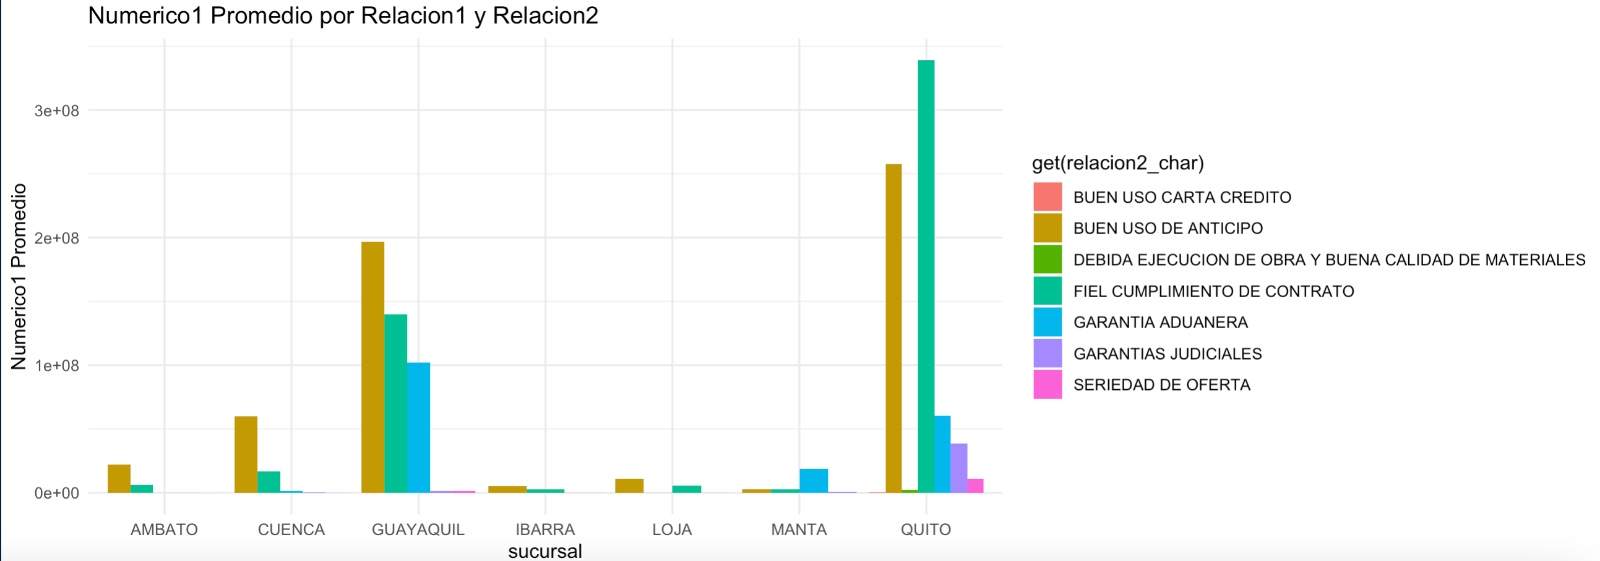
\includegraphics{PHOTO-2024-06-13-15-10-15.jpg}

\subsubsection{Conclusiones e incognitas a primera
vista:}\label{conclusiones-e-incognitas-a-primera-vista}

La relacion entre la sucursal y ramo comercial podemos ver que Quito y
Guayaquil son las sucursales donde mas (en promedio) firmas de contratos
se realizan al menos en dos a tres tipos de ramo comercial, las
siguientes preguntas a realizrse son: -¿Y si mañana sucede un
antecedente donde exigen el contrato de seguro? - ¿Tenemos los fondos
suficientes para sustentar ese gasto? - ¿Podemos seguir financiando? -
¿Por que las sucursales de Quito y Guayaquil son donde mas firman de
contratos? - ¿Debemos aumentar los empleados en las sucursales de Quito
y Guayaquil? - ¿Debemso despeddir gente en las demas sucursales? - ¿Que
estrategia podemos realizar para las demas sucursales? - ¿Tenemos fondo
para abrir otra sucursal en Quito y Guayaquil? - ¿Es necesario abrir
otra sucursal? - ¿Las sucursales sin tantas firmas de contrato
deberiamos cerrarlas? -¿O estan siendo afectadas por la competencia?
-ETC\ldots{}

\subsection{Evaluación de la Evolución Temporal de las
Pólizas.}\label{evaluaciuxf3n-de-la-evoluciuxf3n-temporal-de-las-puxf3lizas.}

\subsubsection{Explicacion del metodo:}\label{explicacion-del-metodo-1}

Se implementó un análisis de series temporales con el objetivo de
comprender el comportamiento de los datos a lo largo del tiempo. Este
estudio permitió identificar patrones y tendencias estacionales que
podrían impactar las decisiones estratégicas de la empresa. Utilizando
modelos de series temporales, se analizaron las fluctuaciones en los
datos, ayudando a prever cambios futuros y a ajustar las estrategias de
negocio acorde a estos hallazgos.

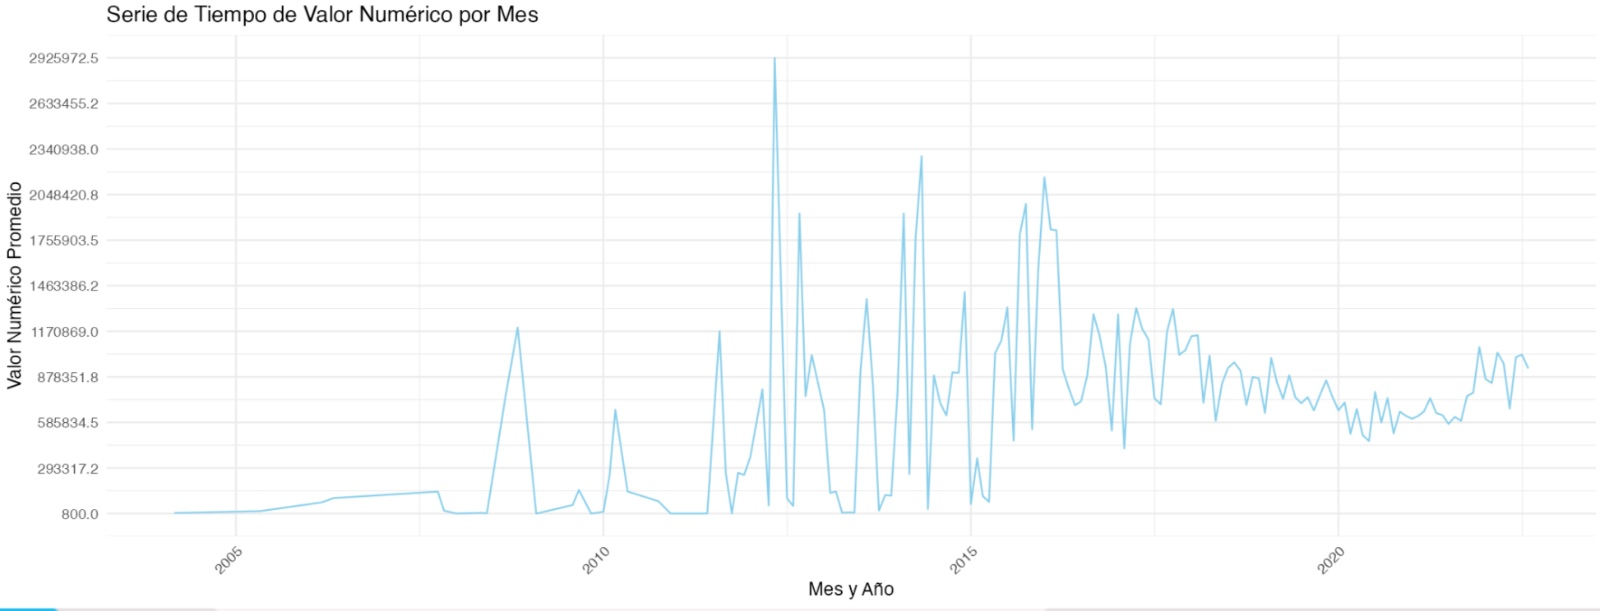
\includegraphics{PHOTO-2024-06-13-15-10-27.jpg}

\subsubsection{Conclusiones e incognitas a primera
vista:}\label{conclusiones-e-incognitas-a-primera-vista-1}

Los graficos estan agrupados por meses notemos que la serie o grafica
tiene picos y pendientes muy macarcados, las preguntas a realizarnos son
las siguientes: -¿Estos picos son en verdad datos atipicos? - ¿Que paso
en el timpo durante la decaida? - ¿A pesar picos podemos ver un aligera
tendencia a la alza, factor a relacionar, inseguridad del pais? - ¿De
investigamos estos picos, fraudes? - ¿Por que tenemos picos que crecen
de manera constante y decrecen de igual forma? - ¿Que tanto lo podemos
relacionar con la inseguridad u otros factores?

\subsection{Segmentación de Clientes por Tipo de Póliza y Monto
Asegurado:}\label{segmentaciuxf3n-de-clientes-por-tipo-de-puxf3liza-y-monto-asegurado}

\subsubsection{Explicacion del metodo:}\label{explicacion-del-metodo-2}

Finalmente, se llevó a cabo un análisis de clustering para segmentar a
los clientes según el tipo de póliza y el monto asegurado. Esta
segmentación se basó en variables clave como el tipo de persona, el tipo
de agente y la suma asegurada. El uso de técnicas de clustering
avanzadas permitió identificar grupos homogéneos de clientes,
facilitando la implementación de estrategias de marketing y ventas más
dirigidas y efectivas.

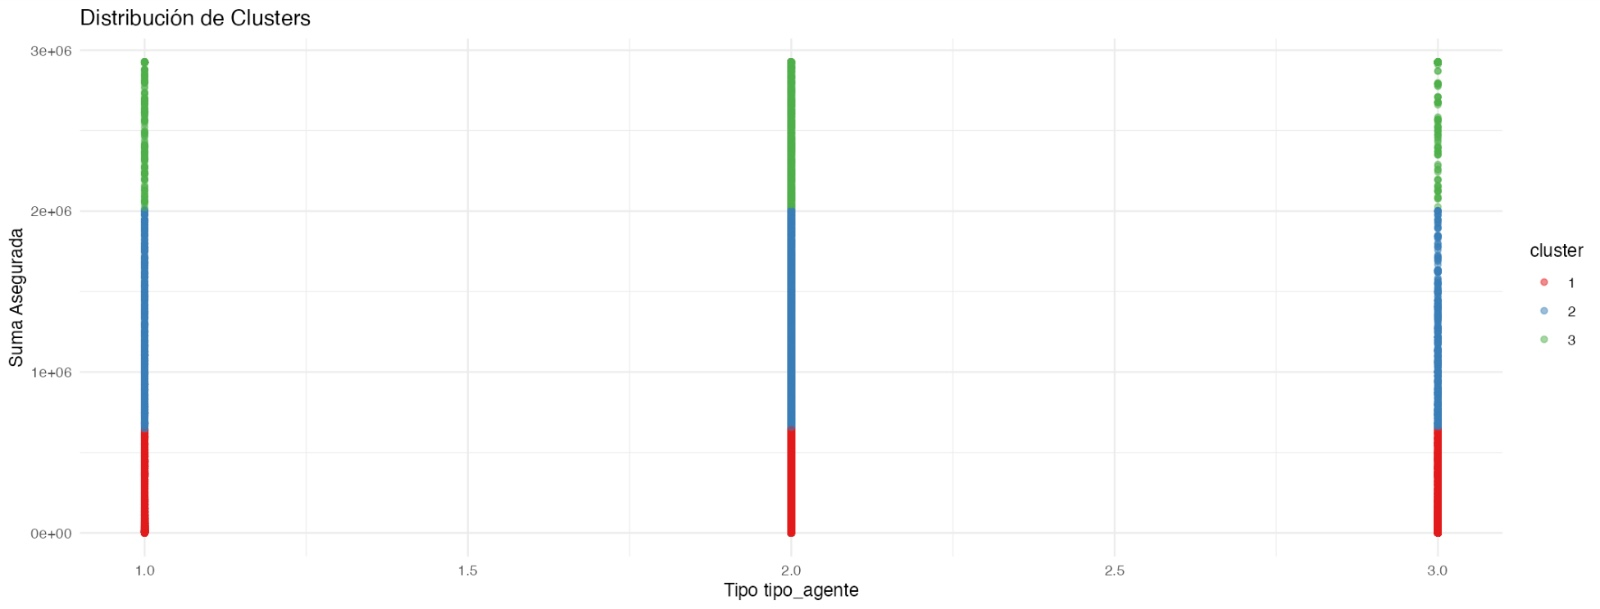
\includegraphics{PHOTO-2024-06-13-15-13-05.jpg}

\subsubsection{Conclusiones:}\label{conclusiones}

Sbemos que el k-means lo que hace es agrupar datos, entonces tenemos un
reduccion en la dimension de los datos, es decir, como son agrupados en
vez de analizar a cada individuo podemos agruparlos y hacer estudios mas
simplificados, por ejemplo, si queremos ver estrategias de marketing
tenemos individuos con caracteristicas comunes donde la estrategia de
publicidad serviria para todo los de ese cluster. De igual manera
tenemos que nos puede a detectar el fraude, nos referimos a que las
desviaciones de patrones pueden ayudar a la deteccion de fraude en caso
de serlo.

\section{Conclusiones generales:}\label{conclusiones-generales}

El breve análisis que hemos realizado ha mejorado nuestra comprensión
del mercado, nuestros servicios y nuestros clientes. Sin embargo, no es
suficiente, ya que hemos dejado muchas preguntas sin responder. Para
abordar estas incógnitas, necesitamos llevar a cabo un análisis más
profundo y orientado a objetivos específicos.

\end{document}
